\documentclass[journal,12pt,twocolumn]{IEEEtran}
\usepackage{setspace}
\usepackage{gensymb}
\usepackage{caption}
%\usepackage{multirow}
%\usepackage{multicolumn}
%\usepackage{subcaption}
%\doublespacing
\usepackage{polynom}
\makeatletter
\def\pld@CF@loop#1+{%
    \ifx\relax#1\else
        \begingroup
          \pld@AccuSetX11%
          \def\pld@frac{{}{}}\let\pld@symbols\@empty\let\pld@vars\@empty
          \pld@false
          #1%
          \let\pld@temp\@empty
          \pld@AccuIfOne{}{\pld@AccuGet\pld@temp
                            \edef\pld@temp{\noexpand\pld@R\pld@temp}}%
           \pld@if \pld@Extend\pld@temp{\expandafter\pld@F\pld@frac}\fi
           \expandafter\pld@CF@loop@\pld@symbols\relax\@empty
           \expandafter\pld@CF@loop@\pld@vars\relax\@empty
           \ifx\@empty\pld@temp
               \def\pld@temp{\pld@R11}%
           \fi
          \global\let\@gtempa\pld@temp
        \endgroup
        \ifx\@empty\@gtempa\else
            \pld@ExtendPoly\pld@tempoly\@gtempa
        \fi
        \expandafter\pld@CF@loop
    \fi}
\def\pld@CMAddToTempoly{%
    \pld@AccuGet\pld@temp\edef\pld@temp{\noexpand\pld@R\pld@temp}%
    \pld@CondenseMonomials\pld@false\pld@symbols
    \ifx\pld@symbols\@empty \else
        \pld@ExtendPoly\pld@temp\pld@symbols
    \fi
    \ifx\pld@temp\@empty \else
        \pld@if
            \expandafter\pld@IfSum\expandafter{\pld@temp}%
                {\expandafter\def\expandafter\pld@temp\expandafter
                    {\expandafter\pld@F\expandafter{\pld@temp}{}}}%
                {}%
        \fi
        \pld@ExtendPoly\pld@tempoly\pld@temp
        \pld@Extend\pld@tempoly{\pld@monom}%
    \fi}
\makeatother
\singlespacing
\usepackage{csvsimple}
\usepackage{amssymb}
\usepackage{amsmath}
\usepackage{multicol}
%\usepackage{enumerate}
\usepackage{amssymb}
%\usepackage{graphicx}
\usepackage{newfloat}
%\usepackage{syntax}
\usepackage{listings}
\usepackage{color}
\usepackage{tikz}
\usepackage{graphicx}
\usetikzlibrary{shapes,arrows}

%\usepackage{graphicx}
%\usepackage{amssymb}
%\usepackage{relsize}
%\usepackage[cmex10]{amsmath}
%\usepackage{mathtools}
%\usepackage{amsthm}
%\interdisplaylinepenalty=2500
%\savesymbol{iint}
%\usepackage{txfonts}
%\restoresymbol{TXF}{iint}
%\usepackage{wasysym}
\usepackage{amsthm}
\usepackage{mathrsfs}
\usepackage{txfonts}
\usepackage{stfloats}
\usepackage{cite}
\usepackage{cases}
\usepackage{mathtools}
\usepackage{caption}
\usepackage{enumerate}	
\usepackage{enumitem}
\usepackage{amsmath}
%\usepackage{xtab}
\usepackage{longtable}
\usepackage{multicol}
\usepackage{multirow}
%\usepackage{algorithm}
%\usepackage{algpseudocode}
\usepackage{enumitem}
\usepackage{mathtools}
\usepackage{hyperref}
%\usepackage[framemethod=tikz]{mdframed}
\usepackage{listings}
    %\usepackage[latin1]{inputenc}                                 %%
    \usepackage{color}                                            %%
    \usepackage{array}                                            %%
    \usepackage{longtable}                                        %%
    \usepackage{calc}                                             %%
    \usepackage{multirow}                                         %%
    \usepackage{hhline}                                           %%
    \usepackage{ifthen}                                           %%
  %optionally (for landscape tables embedded in another document): %%
    \usepackage{lscape}     


\usepackage{url}
\def\UrlBreaks{\do\/\do-}


%\usepackage{stmaryrd}


%\usepackage{wasysym}
%\newcounter{MYtempeqncnt}
\DeclareMathOperator*{\Res}{Res}
%\renewcommand{\baselinestretch}{2}
\renewcommand\thesection{\arabic{section}}
\renewcommand\thesubsection{\thesection.\arabic{subsection}}
\renewcommand\thesubsubsection{\thesubsection.\arabic{subsubsection}}

\renewcommand\thesectiondis{\arabic{section}}
\renewcommand\thesubsectiondis{\thesectiondis.\arabic{subsection}}
\renewcommand\thesubsubsectiondis{\thesubsectiondis.\arabic{subsubsection}}

% correct bad hyphenation here
\hyphenation{op-tical net-works semi-conduc-tor}

%\lstset{
%language=C,
%frame=single, 
%breaklines=true
%}

%\lstset{
	%%basicstyle=\small\ttfamily\bfseries,
	%%numberstyle=\small\ttfamily,
	%language=Octave,
	%backgroundcolor=\color{white},
	%%frame=single,
	%%keywordstyle=\bfseries,
	%%breaklines=true,
	%%showstringspaces=false,
	%%xleftmargin=-10mm,
	%%aboveskip=-1mm,
	%%belowskip=0mm
%}

%\surroundwithmdframed[width=\columnwidth]{lstlisting}
\def\inputGnumericTable{}                                 %%
\lstset{
%language=C,
frame=single, 
breaklines=true,
columns=fullflexible
}

\begin{document}
%
\tikzstyle{block} = [rectangle, draw,
    text width=3em, text centered, minimum height=3em]
\tikzstyle{sum} = [draw, circle, node distance=3cm]
\tikzstyle{input} = [coordinate]
\tikzstyle{output} = [coordinate]
\tikzstyle{pinstyle} = [pin edge={to-,thin,black}]

\theoremstyle{definition}
\newtheorem{theorem}{Theorem}[section]
\newtheorem{problem}{Problem}
\newtheorem{proposition}{Proposition}[section]
\newtheorem{lemma}{Lemma}[section]
\newtheorem{corollary}[theorem]{Corollary}
\newtheorem{example}{Example}[section]
\newtheorem{definition}{Definition}[section]
%\newtheorem{algorithm}{Algorithm}[section]
%\newtheorem{cor}{Corollary}
\newcommand{\BEQA}{\begin{eqnarray}}
\newcommand{\EEQA}{\end{eqnarray}}
\newcommand{\define}{\stackrel{\triangle}{=}}

\bibliographystyle{IEEEtran}
%\bibliographystyle{ieeetr}

\providecommand{\nCr}[2]{\,^{#1}C_{#2}} % nCr
\providecommand{\nPr}[2]{\,^{#1}P_{#2}} % nPr
\providecommand{\mbf}{\mathbf}
\providecommand{\mtx}[1]{\mathbf{#1}}
\providecommand{\pr}[1]{\ensuremath{\Pr\left(#1\right)}}
\providecommand{\qfunc}[1]{\ensuremath{Q\left(#1\right)}}
\providecommand{\sbrak}[1]{\ensuremath{{}\left[#1\right]}}
\providecommand{\lsbrak}[1]{\ensuremath{{}\left[#1\right.}}
\providecommand{\rsbrak}[1]{\ensuremath{{}\left.#1\right]}}
\providecommand{\brak}[1]{\ensuremath{\left(#1\right)}}
\providecommand{\lbrak}[1]{\ensuremath{\left(#1\right.}}
\providecommand{\rbrak}[1]{\ensuremath{\left.#1\right)}}
\providecommand{\cbrak}[1]{\ensuremath{\left\{#1\right\}}}
\providecommand{\lcbrak}[1]{\ensuremath{\left\{#1\right.}}
\providecommand{\rcbrak}[1]{\ensuremath{\left.#1\right\}}}
\theoremstyle{remark}
\newtheorem{rem}{Remark}
\newcommand{\sgn}{\mathop{\mathrm{sgn}}}
\providecommand{\ztrans}{\overset{\mathcal{Z}}{ \rightleftharpoons}}
\providecommand{\abs}[1]{\left\vert#1\right\vert}
\providecommand{\res}[1]{\Res\displaylimits_{#1}} 
\providecommand{\norm}[1]{\left\Vert#1\right\Vert}
\providecommand{\mtx}[1]{\mathbf{#1}}
\providecommand{\pd}[2]{\ensuremath{\frac{\partial #1}{\partial #2}}}
\providecommand{\mean}[1]{E\left[ #1 \right]}
\providecommand{\fourier}{\overset{\mathcal{F}}{ \rightleftharpoons}}
\providecommand{\gauss}[2]{\mathcal{N}\ensuremath{\left(#1,#2\right)}}
%\providecommand{\hilbert}{\overset{\mathcal{H}}{ \rightleftharpoons}}
\providecommand{\system}{\overset{\mathcal{H}}{ \longleftrightarrow}}
%\newcommand{\solution}[2]{\textbf{Solution:}{#1}}
\newcommand{\solution}{\noindent \textbf{Solution: }}
\newcommand{\myvec}[1]{\ensuremath{\begin{pmatrix}#1\end{pmatrix}}}
\newcommand{\sqvec}[1]{\ensuremath{\left[\begin{array}{c}#1\end{array}\right]}}
\providecommand{\dec}[2]{\ensuremath{\overset{#1}{\underset{#2}{\gtrless}}}}
\DeclarePairedDelimiter{\ceil}{\lceil}{\rceil}
%\numberwithin{equation}{section}
%\numberwithin{problem}{subsection}
%\numberwithin{definition}{subsection}
\makeatletter
\@addtoreset{figure}{section}
\makeatother

\let\StandardTheFigure\thefigure
%\renewcommand{\thefigure}{\theproblem.\arabic{figure}}
\renewcommand{\thefigure}{\thesection}


%\numberwithin{figure}{subsection}

%\numberwithin{equation}{subsection}
%\numberwithin{equation}{section}
%\numberwithin{equation}{problem}
%\numberwithin{problem}{subsection}
\numberwithin{problem}{section}
%%\numberwithin{definition}{subsection}
%\makeatletter
%\@addtoreset{figure}{problem}
%\makeatother
\makeatletter
\@addtoreset{table}{section}
\makeatother

\let\StandardTheFigure\thefigure
\let\StandardTheTable\thetable
\let\vec\mathbf
\numberwithin{equation}{section}

\vspace{3cm}


\title{%Convex Optimization in Python
	Filter-Sounds
}
%\title{
%	\logo{Matrix Analysis through Octave}{\begin{center}\includegraphics[scale=.24]{tlc}\end{center}}{}{HAMDSP}
%}

% paper title
% can use linebreaks \\ within to get better formatting as desired
%\title{Matrix Analysis through Octave}
%
%
% author names and IEEE memberships
% note positions of commas and nonbreaking spaces ( ~ ) LaTeX will not break
% a structure at a ~ so this keeps an author's name from being broken across
% two lines.
% use \thanks{} to gain access to the first footnote area
% a separate \thanks must be used for each paragraph as LaTeX2e's \thanks
% was not built to handle multiple paragraphs
%

\author{JARPULA BHANU PRASAD - AI21BTECH11015}
\maketitle

\tableofcontents

\bigskip

\renewcommand{\thefigure}{\theenumi}
\renewcommand{\thetable}{\theenumi}

\begin{abstract}
This manual provides a simple introduction to digital signal processing.
\end{abstract}
%%
\section{Software installation}

\begin{enumerate}[label=\thesection.\arabic*
,ref=\thesection.\theenumi]
\item Run the following commands.
\begin{lstlisting}
sudo apt-get update
sudo apt-get install libffi-dev libsndfile1 python3-scipy python3-numpy python3-matplotlib
sudo pip install cffi pysoundfile
\end{lstlisting}
\end{enumerate}

\section{Digital Filter}

\begin{enumerate}[label=\thesection.\arabic*
,ref=\thesection.\theenumi]
\item Download the sound file from
\begin{lstlisting}
wget https://github.com/jarpula-Bhanu/EE3900/blob/main/Filter/soundfiles/Sound_Noise.wav
\end{lstlisting}

\item You will find a spectogram at https://academo.org/demos/spectrum-analyzer. Upload the sound file that you downloaded in problem 2.1 in the spectrogram and play. Observe the spectogram. What do you find?
\solution There are a lot of yellow lines betweeen 440Hz to 5.1KHz. These represent the synthesizer key tones. Also, the key strokes are audible along with background noise.

\item Write the python code for removal of out of band nosie and execute the code.\label{2.3}\\
\solution Download and run the following code.
\begin{lstlisting}
wget https://github.com/jarpula-Bhanu/EE3900/blob/main/Filter/Codes/2.3_noise.py
\end{lstlisting}
run the above code using the command
\begin{lstlisting}
	python3 2.3_noise.py
\end{lstlisting}

\item The output of the python scripy in problem 2.3 is the audio file Sound\_With\_ReducedNoise.wav. Play the file in the spectogram in problem 2.2. What do you observe?\\
\solution The key strokes as well as background noise is subdued in the audio. Also the signal is blank for frequencies above 5.1KHz.
\end{enumerate}


\section{Difference Equation}

\begin{enumerate}[label=\thesection.\arabic*
,ref=\thesection.\theenumi]
\item Let 
\begin{align}\label{3.1}
	x(n) = \cbrak{\underset{\uparrow}{1},2,3,4,2,1}
\end{align}
Sketch x(n).\\
\solution Download and run the following code.Below code plots fig\eqref{fig:3.1}
\begin{lstlisting}
wget https://github.com/jarpula-Bhanu/EE3900/blob/main/Filter/Codes/3.1.py
\end{lstlisting}
run the above code using the command
\begin{lstlisting}
	python3 3.1.py
\end{lstlisting}
\begin{figure}[h]
    \centering
    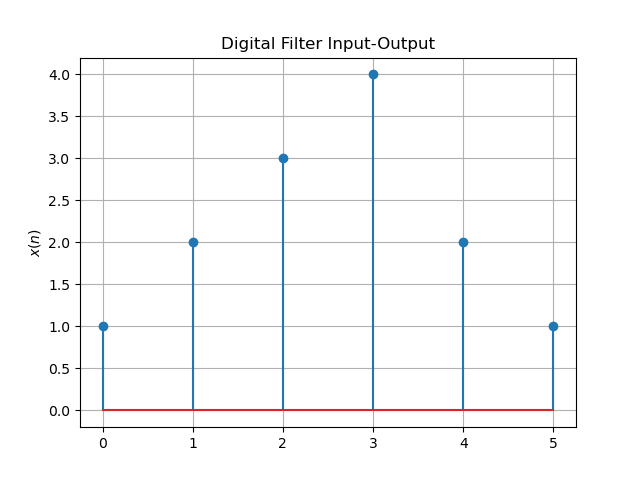
\includegraphics[width=\columnwidth]{./figs/3.1.png}
    \caption{Sketch of $x(n)$}
    \label{fig:3.1}
\end{figure}

\item Let
	\begin{align}\label{3.2}
		y(n) + \frac{1}{2}y(n-1) = x(n)+x(n-2),
		y(n)=0,n<0
	\end{align}
Sketech y(n).\\
\solution Download and run the following code.Below code plots fig\eqref{fig:3.2}
\begin{lstlisting}
wget https://github.com/jarpula-Bhanu/EE3900/blob/main/Filter/Codes/3.2.py
\end{lstlisting}
run the above code using the command
\begin{lstlisting}
	python3 3.2.py
\end{lstlisting}
\begin{figure}[h]
    \centering
    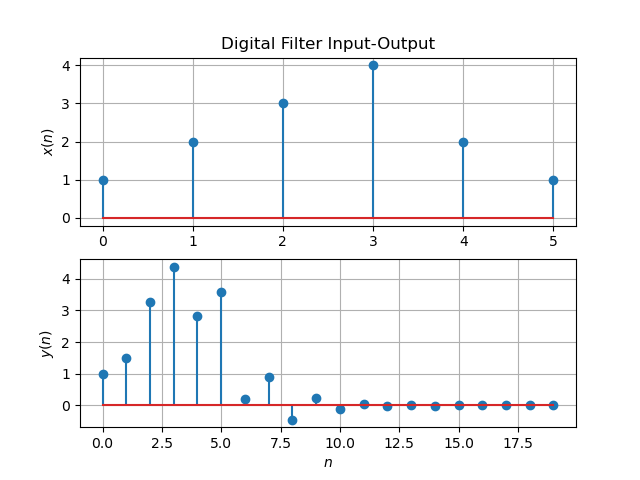
\includegraphics[width=\columnwidth]{./figs/3.2.png}
    \caption{Sketch of $x(n)$ and $y(n)$}
    \label{fig:3.2}
\end{figure}

\item Repeat the above exercise using C code.\\
\solution Download and run the following code.Below code plots fig\eqref{fig:3.3}
\begin{lstlisting}
wget https://github.com/jarpula-Bhanu/EE3900/blob/main/Filter/Codes/3.3.c
wget https://github.com/jarpula-Bhanu/EE3900/blob/main/Filter/Codes/3.3_plot.py
\end{lstlisting}
run the above code using the command
\begin{lstlisting}
	gcc 3.3.c -o 3.3.out
	./3.3.out
	python3 3.3_plot.py
\end{lstlisting}
\begin{figure}[h]
    \centering
    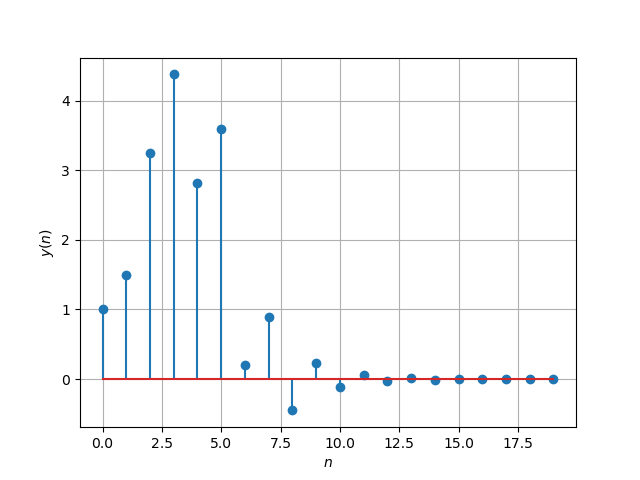
\includegraphics[width=\columnwidth]{./figs/3.3_plot.png}
    \caption{Sketch of $y(n)$}
    \label{fig:3.3}
\end{figure}


\end{enumerate}

\section{$Z$-transform}

\begin{enumerate}[label=\thesection.\arabic*
,ref=\thesection.\theenumi]
\item The Z-transform of $x(n)$ is defined as 
\begin{align}\label{4.1}
	X(z) = \mathcal{Z}\cbrak{x(n)} = \sum_{n=-\infty}^\infty x(n) z^{-n}
\end{align}
Show that
\begin{align}\label{4.2}
	\mathcal{Z}\cbrak{x(n-1)} = z^{-1}X(z)
\end{align}
and find
\begin{align}
	\mathcal{Z}\cbrak{x(n-k)}
\end{align}
\solution From \eqref{4.1}
\begin{align}
	\mathcal{Z}\cbrak{x(n-k)} &= \sum_{n=-\infty}^\infty x(n-1)z^{-n}\\
	&= \sum_{n=-\infty}^\infty x(n)z^{-n-1}= z^{-1}\sum_{n=-\infty}^\infty x(n)z^{-n}
\end{align}
resulting in \eqref{4.2}. Similarly, it can be shown that 
\begin{align}\label{4.6}
	\mathcal{Z}\cbrak{x(n-k)} = z^{-k}X(z)
\end{align}

$\mathcal{Z}$- transform of $x(n)$ is 

\begin{align}
\mathcal{Z}\cbrak{x(n)} &= 1+2 z^{-1}+3 z^{-2} + 4 z^{-3} + 2 z^{-4} + z^{-5}
\end{align}

\begin{align}
\mathcal{Z}\cbrak{x(n-k)} &= z^{-k}(1+2 z^{-1}+3 z^{-2} +\\&\hspace*{10mm} 4 z^{-3} + 2 z^{-4} + z^{-5})\\
\mathcal{Z}\cbrak{x(n-k)} &= z^{-k}+2 z^{-(k+1)}+3 z^{-(k+2)} \\&+ 4 z^{-(k+3)} + 2 z^{-(k+4)} + z^{-(k+5)}
\end{align}

\item Obtain $X(z)$ for $x(n)$ in problem \eqref{3.1}\\
\solution \begin{align}
	\mathcal{Z}\cbrak{x(n)} &= 1+2 z^{-1}+3 z^{-2} + 4 z^{-3} + 2 z^{-4} + z^{-5}
	\end{align}
	
	\begin{align}
	\mathcal{Z}\cbrak{x(n-k)} &= z^{-k}(1+2 z^{-1}+3 z^{-2} +\\&\hspace*{10mm} 4 z^{-3} + 2 z^{-4} + z^{-5})\\
	\mathcal{Z}\cbrak{x(n-k)} &= z^{-k}+2 z^{-(k+1)}+3 z^{-(k+2)} \\&+ 4 z^{-(k+3)} + 2 z^{-(k+4)} + z^{-(k+5)}
	\end{align}
\item Find
%
\begin{equation}\label{4.7}
H(z) = \frac{Y(z)}{X(z)}
\end{equation}
%
from  \eqref{3.2} assuming that the $Z$-transform is a linear operation.
\\
\solution  Applying \eqref{4.6} in \eqref{3.2},
\begin{align}\label{4.9}
Y(z) + \frac{1}{2}z^{-1}Y(z) &= X(z)+z^{-2}X(z)
\\
\implies \frac{Y(z)}{X(z)} &= \frac{1 + z^{-2}}{1 + \frac{1}{2}z^{-1}}
\label{eq:freq_resp}
\end{align}
%
\item Find the Z transform of 
\begin{equation}
\delta(n)
=
\begin{cases}
1 & n = 0
\\
0 & \text{otherwise}
\end{cases}
\end{equation}
and show that the $Z$-transform of
\begin{equation}
\label{eq:unit_step}
u(n)
=
\begin{cases}
1 & n \ge 0
\\
0 & \text{otherwise}
\end{cases}
\end{equation}
is
\begin{equation}
U(z) = \frac{1}{1-z^{-1}}, \quad \abs{z} > 1
\end{equation}
\solution It is easy to show that
\begin{equation}
\delta(n) \ztrans 1
\end{equation}
and from \eqref{eq:unit_step},
\begin{align}
U(z) &= \sum _{n= 0}^{\infty}z^{-n}
\\
&=\frac{1}{1-z^{-1}}, \quad \abs{z} > 1
\end{align}
using the fomula for the sum of an infinite geometric progression.
%
\item Show that 
\begin{equation}
\label{eq:anun}
a^nu(n) \ztrans \frac{1}{1-az^{-1}} \quad \abs{z} > \abs{a}
\end{equation}
\solution \begin{align}
	a^nu(n) &\ztrans \sum_{n=0}^\infty (az^{-1})^n\\
	& =\frac{1}{1-az^{-1}} \quad \abs{z} > \abs{a}
\end{align}
%
\item 
Let
\begin{equation}
H\brak{e^{j \omega}} = H\brak{z = e^{j \omega}}.
\end{equation}
Plot $\abs{H\brak{e^{j \omega}}}$.  Comment.  $H(e^{j \omega})$ is
known as the {\em Discret Time Fourier Transform} (DTFT) of $x(n)$.
\\
\solution Download and run the following code. The following code plots Fig. \ref{fig:dtft}.
\begin{lstlisting}
wget https://github.com/jarpula-Bhanu/EE3900/blob/main/Filter/Codes/4.5.py
\end{lstlisting}
run the above code using the command 
\begin{lstlisting}
	python3 4.5.py
\end{lstlisting}
We observe that $\abs{H\brak{e^{j \omega}}}$ is periodic with fundamental period $2\pi$.
\begin{figure}[!ht]
\centering
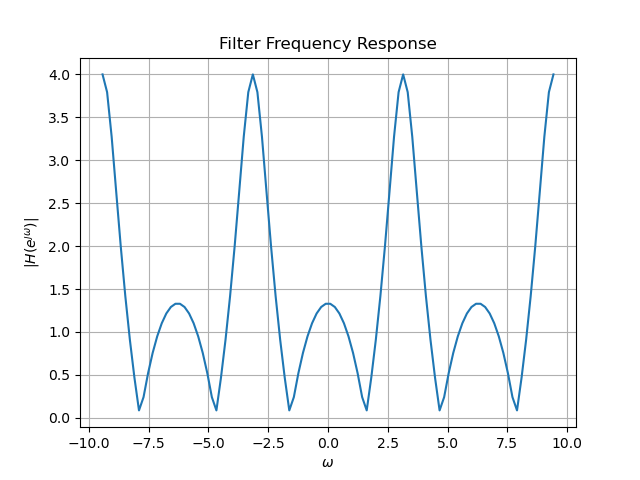
\includegraphics[width=\columnwidth]{./figs/4.5.png}
\caption{$\abs{H\brak{e^{j\omega}}}$}
\label{fig:dtft}
\end{figure}

\begin{align}
	H\brak{e^{j \omega}} &= \frac{1 + e^{-2j\omega}}{1 + \frac12 e^{-j\omega}} \\
	\implies \abs{H\brak{e^{j \omega}}} &= \frac{\abs{1 + \cos2\omega - j\sin2\omega}}{\abs{1 + \frac12 \cos\omega - \frac12 \sin\omega}} \\
	&= \sqrt{\frac{(1 + \cos2\omega)^2 + (\sin2\omega)^2}{(1 + \frac12 \cos\omega)^2 + (\frac12 \sin\omega)^2}} \\
	&= \sqrt{\frac{2 + 2\cos2\omega}{\frac54 + \cos\omega}} \\
	&= \sqrt{\frac{2(2\cos^2\omega)4}{5 + 4\cos\omega} } \\
	&= \frac{4\abs{\cos\omega}}{\sqrt{5 + 4\cos\omega}}
\end{align}

period of $\abs{cos \omega}$ is $\pi$ and period of $\sqrt{5 + 4\cos \omega}$ is $2\pi$.\\
Now period of $\abs{H\brak{e^{j \omega}}}$ is $\frac{LCM(\pi,2\pi)}{HCF(\pi,2\pi)}$ = $\frac{2\pi}{1}$ = $2\pi$\\

\item Express $h(n)$ in terms of $H(e^{j\omega})$\\
\solution $h(n)$ is given by the inverse DTFT of $H(e^{j\omega})$
\begin{align}
	h(n) &= \frac{1}{2\pi}\int_{-\pi}^\pi H(e^{j\omega})e^{j\omega n}d\omega\\
	&=\frac{1}{2\pi}\sum_{n=-\infty}^\infty\int_{-\pi}^\pi h(k)e^{-j\omega k} e^{j\omega n} d\omega \\
	&=\frac{1}{2\pi}\sum_{n=-\infty}^\infty h(k)\int_{-\pi}^{\pi}e^{j\omega(n-k)}d\omega \\
	&= \frac{1}{2\pi}\sum_{n=-\infty}^\infty h(k) 2\pi \delta[n-k]\\
	&=h(n)
\end{align}
Since 
\begin{align}
	\int_{-\pi}^{\pi}e^{j\omega n}d\omega &=2\pi \delta[n]\\
	and \\
	\delta[n-k]&=
	\begin{cases}
		1 & n =k
		\\
		0 & \text{otherwise}
	\end{cases}
\end{align}



\end{enumerate}

\section{Impulse Response}

\begin{enumerate}[label=\thesection.\arabic*
,ref=\thesection.\theenumi]
\item Using long division, find
\begin{align}
	h(n), \quad n < 5
\end{align}
for $H(z)$ in \eqref{eq:freq_resp}

\solution 
\begin{equation}
	H(z) = \frac{1 + z^{-2}}{1 + \frac12 z^{-1}}
\end{equation}
Substitute $z^{-1} = x$

\polylongdiv{1+x^2}{1+\frac12 x}

\begin{align}
	&\implies 1 + z^{-2} = \brak{1 + \frac12 z^{-1}}\brak{-4 + 2z^{-1}} + 5 \\
	&\implies H(z) = -4 + 2z^{-1} + \frac{5}{1 + \frac12 z^{-1}}
\end{align}

\begin{align}
	\frac{5}{1 + \frac12 z^{-1}} &= 5 \brak{1 + \frac12 z^{-1}}^{-1} \\
	&= 5 \sum_{n=0}^\infty \brak{-\frac{z^{-1}}{2}}^n
\end{align}

\begin{multline}
	H(z) = -4 + 2z^{-1} + 5 - \frac{5}{2}z^{-1} + \frac{5}{4}z^{-2}\\ - \frac{5}{8}z^{-3}  + \frac{5}{16}z^{-4} - \frac{5}{32}z^{-5} + \cdots
\end{multline}

\begin{align}
	H(z) = -4 + 2z^{-1}+5\brak{-\frac{1}{2}}^{n-2}  \text{for $n\ge2$} 
\end{align}

Therefore, by comparing coefficients
\begin{align}
	h(n) = 
	\begin{cases}
		1 & n = 0 \\
		-\dfrac12 & n = 1 \\
		\dfrac{5}{4} & n = 2 \\
		-\dfrac{5}{8} & n = 3 \\
		\dfrac{5}{16} & n = 4 \\
	\end{cases}
\end{align}

Alternatively, on applying the inverse $Z$-transform on both sides of the equation
\begin{align}
	H(z) &\ztrans h(n) \\
	-4 &\ztrans -4\delta(n) \\
	2z^{-1} &\ztrans 2\delta(n - 1) \\
	\frac{5}{1 + \frac12 z^{-1}} &\ztrans 5\brak{-\frac12}^n u(n) \\
\end{align}

Therefore,
\begin{equation}
	h(n) = -4\delta(n) + 2\delta(n - 1) + 5\brak{-\frac12}^n u(n)
\end{equation}

Download the following Python code that plots Fig. \ref{fig-5.1}.
\begin{lstlisting}
wget https://github.com/jarpula-Bhanu/EE3900/blob/main/Filter/Codes/5.1.py
\end{lstlisting}

Run the code by executing
\begin{lstlisting}
	python 5.1.py
\end{lstlisting}

\begin{figure}[!ht]
	\centering
	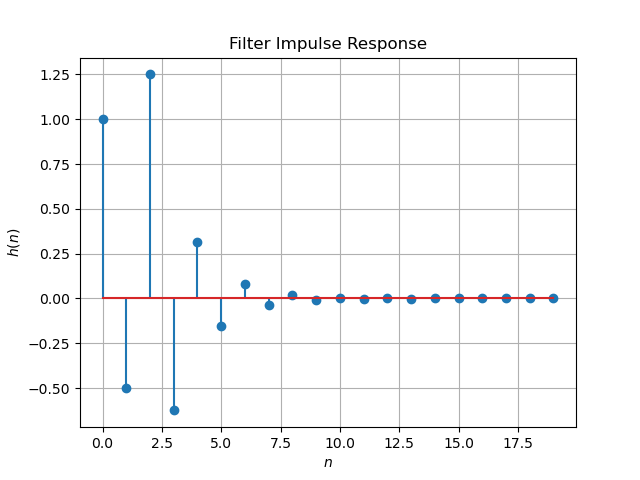
\includegraphics[width=\columnwidth]{./figs/5.1.png}
	\caption{Plot of $h(n)$}
	\label{fig-5.1}	
\end{figure} 
\item \label{prob:impulse_resp}
Find an expression for $h(n)$ using $H(z)$, given that 
%in Problem \ref{eq:ztransab} and \eqref{eq:anun}, given that
\begin{equation}
\label{eq:impulse_resp}
h(n) \ztrans H(z)
\end{equation}
and there is a one to one relationship between $h(n)$ and $H(z)$. $h(n)$ is known as the {\em impulse response} of the
system defined by \eqref{3.2}.
\\
\solution From \eqref{eq:freq_resp},
\begin{align}
H(z) &= \frac{1}{1 + \frac{1}{2}z^{-1}} + \frac{ z^{-2}}{1 + \frac{1}{2}z^{-1}}
\\
\implies h(n) &= \brak{-\frac{1}{2}}^{n}u(n) + \brak{-\frac{1}{2}}^{n-2}u(n-2)
\end{align}
using \eqref{eq:anun} and \eqref{4.6}.
\item Sketch $h(n)$. Is it bounded? Justify theoretically.
\\
\solution Download and run the following code.The following code plots Fig. \ref{fig:hn}.
\begin{lstlisting}
wget https://github.com/jarpula-Bhanu/EE3900/blob/main/Filter/Codes/5.2.py
\end{lstlisting}
run the above code using the command.
\begin{lstlisting}
	python3 5.2.py
\end{lstlisting}
\begin{figure}[!ht]
\centering
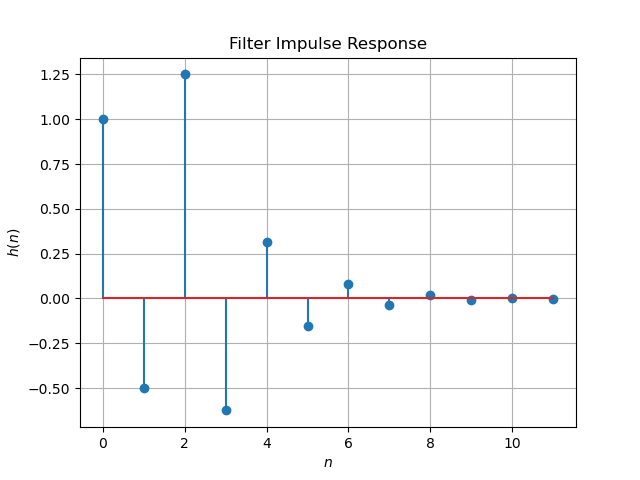
\includegraphics[width=\columnwidth]{./figs/5.2.png}
\caption{$h(n)$ as the inverse of $H(z)$}
\label{fig:hn}
\end{figure}
From the plot, it is clear that $h(n)$ is bounded. Theoretically,
	\begin{align}
		\abs{u(n)} &\le 1 \\
		\abs{\brak{-\frac12}^n} &\le 1 \\
		\implies \abs{\brak{-\frac12}^n u(n)} &\le 1
	\end{align}
	
	Similarly,
	\begin{align}
		\abs{\brak{-\frac12}^{n-2} u(n-2)} &\le 1 \\
		\implies h(n) &\le 2
	\end{align}
	
	Therefore $h(n)$ is bounded.
%
\item Convergent? Justify using the ratio test.\label{bounded}\\
\solution The ratio test for convergence
\begin{align}
	\lim_{n \to \infty} \abs{\frac{h(n+1)}{h(n)}} &= \lim_{n \to \infty} \abs{\frac{\brak{-\frac12}^{n-1} \brak{\frac14 + 1}}{\brak{-\frac12}^{n-2} \brak{\frac14 + 1}}} \\
	&= \lim_{n \to \infty} \abs{-\frac12} \\
	&= \frac{1}{2} < 1
\end{align}

Therefore, $h(n)$ is convergent which implies that it is bounded.
\item The system with $h(n)$ is defined to be stable if
\begin{equation}
\sum_{n=-\infty}^{\infty}h(n) < \infty
\end{equation}
Is the system defined by \eqref{3.2} stable for the impulse response in \eqref{eq:impulse_resp}?\\
%
\solution Note that
\begin{align}
	\sum_{n=-\infty}^\infty h(n) &= \sum_{n=-\infty}^\infty \brak{-\frac{1}{2}}^nu(n)+\brak{-\frac{1}{2}}^{n-2}u(n-2)\\
	&= 2\brak{\frac{1}{1+\frac{1}{2}}} = \frac{4}{3}
\end{align}
Thus, the given system is stable.
\item Verify the above result using a python code.\\
\solution Download the following code.
\begin{lstlisting}
wget https://github.com/jarpula-Bhanu/EE3900/blob/main/Filter/Codes/5.6.py
\end{lstlisting}

Run the code by executing
\begin{lstlisting}
	python 5.6.py
\end{lstlisting}

\item Compute and sketch $h(n)$ using 
\begin{equation}
\label{eq:iir_filter_h}
h(n) + \frac{1}{2}h(n-1) = \delta(n) + \delta(n-2), 
\end{equation}
%
This is the definition of $h(n)$.
\\
\solution The following code plots Fig. \ref{fig:hndef}. Note that this is the same as Fig. 
\ref{fig:hn}. 
%
\begin{lstlisting}
wget https://github.com/jarpula-Bhanu/EE3900/blob/main/Filter/Codes/5.4.py
\end{lstlisting}
run the above code using the command.
\begin{lstlisting}
	python3 5.4.py
\end{lstlisting}
\begin{figure}[!ht]
\centering
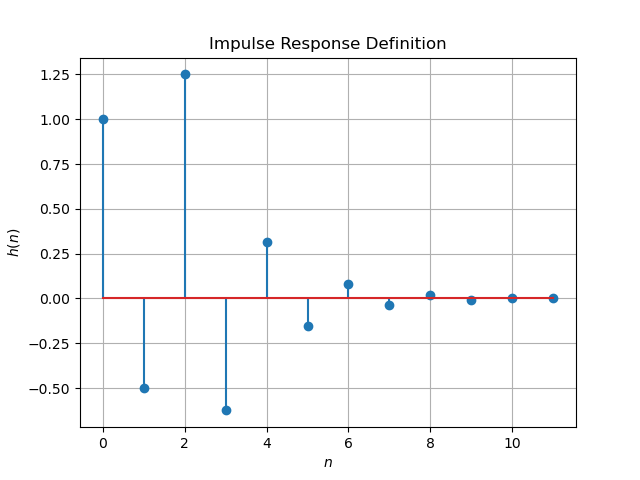
\includegraphics[width=\columnwidth]{./figs/5.4.png}
\caption{$h(n)$ from the definition}
\label{fig:hndef}
\end{figure}
%
\item Compute 
%
\begin{equation}
\label{eq:convolution}
y(n) = x(n)*h(n) = \sum_{n=-\infty}^{\infty}x(k)h(n-k)
\end{equation}
%
Comment. The operation in \eqref{eq:convolution} is known as
{\em convolution}.
%
\\
\solution The following code plots Fig. \ref{fig:ynconv}. Note that this is the same as 
$y(n)$ in  Fig. 
\ref{fig:3.2}. 
%
\begin{lstlisting}
wget https://github.com/jarpula-Bhanu/EE3900/blob/main/Filter/Codes/5.5.py
\end{lstlisting}
run the above code using the command.
\begin{lstlisting}
	python3 5.5.py
\end{lstlisting}
\begin{figure}[!ht]
\centering
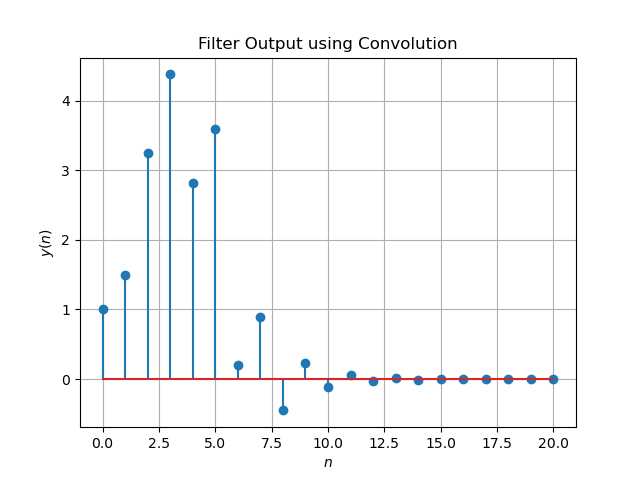
\includegraphics[width=\columnwidth]{./figs/5.5.png}
\caption{$y(n)$ from the definition of convolution}
\label{fig:ynconv}
\end{figure}
\item Express the above convolution using a Teoplitz matrix.\\
\solution  Let 
\begin{align}
	\vec{x} = \myvec{1 \\ 2 \\ 3 \\ 4 \\ 2 \\ 1} \qquad
	\vec{h} = \myvec{1 \\ -0.5 \\ 1.25 \\ -0.62 \\ 0.31 \\ -0.16}
\end{align}

Their convolution is given by the product of the following Toeplitz matrix $\vec{T}$
\begin{align}
	&\myvec{
		1 & 0 & 0 & 0 & 0 & 0 \\
		-0.5 & 1 & 0 & 0 & 0 & 0 \\
		1.25 & -0.5 & 1 & 0 & 0 & 0 \\
		-0.62 & 1.25 & -0.5 & 1 & 0 & 0 \\
		0.31 & -0.62 & 1.25 & -0.5 & 1 & 0 \\
		-0.16 & 0.31 & -0.62 & 1.25 & -0.5 & 1 \\
		0 & -0.16 & 0.31 & -0.62 & 1.25 & -0.5 \\
		0 & 0 & -0.16 & 0.31 & -0.62 & 1.25 \\
		0 & 0 & 0 & -0.16 & 0.31 & -0.62 \\
		0 & 0 & 0 & 0 & -0.16 & 0.31 \\
		0 & 0 & 0 & 0 & 0 & -0.16 \\
	} 
\end{align}
and $\vec{x}$

\begin{align}
	&\vec{y} = \vec{x} \circledast \vec{h} = \vec{Tx} = \myvec{1 \\ 1.5 \\ 3.25 \\ 4.38 \\ 2.81 \\ 3.59 \\ 0.12 \\ 0.78 \\ -0.62 \\ 0 \\ -0.16}
\end{align}
Download the following code .
\begin{lstlisting}
wget https://github.com/jarpula-Bhanu/EE3900/blob/main/Filter/Codes/5.9.py
\end{lstlisting}

Run the code by executing
\begin{lstlisting}
	python 5.9.py
\end{lstlisting}
\begin{figure}[!ht]
	\centering
	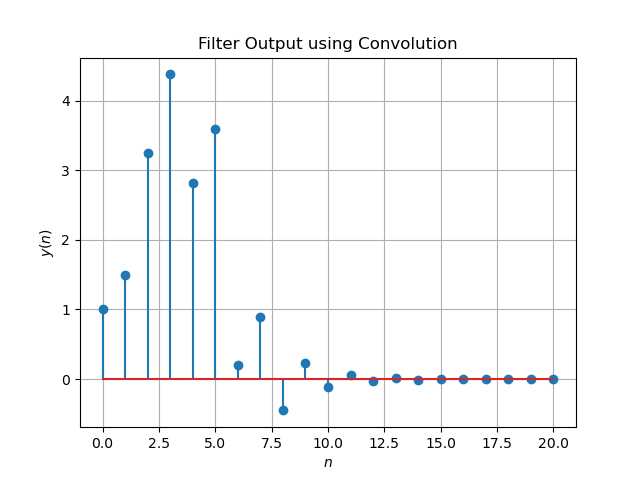
\includegraphics[width=\columnwidth]{./figs/5.5_conv.png}
	\caption{Plot of the convolution of $x(n)$ and $h(n)$}
	\label{fig-5.5-toeplitz}	
\end{figure}

\item Show that 
\begin{equation}
y(n) =  \sum_{n=-\infty}^{\infty}x(n-k)h(k)
\end{equation}
\solution from \ref{eq:convolution}, we substitute $k := n-k$ to get
\begin{align}
	y(n) &= \sum_{k=-\infty}^\infty x(k)h(n-k)\\
	&= \sum_{n-k=-\infty}^\infty x(n-k)h(k)\\
	&= \sum_{k=-\infty}^\infty x(n-k)h(k)
\end{align}

\end{enumerate}

\section{DFT and FFT}

\begin{enumerate}[label=\thesection.\arabic*
,ref=\thesection.\theenumi]
\item
Compute
\begin{equation}
X(k) \define \sum _{n=0}^{N-1}x(n) e^{-\j2\pi kn/N}, \quad k = 0,1,\dots, N-1
\end{equation}
and $H(k)$ using $h(n)$.\\
\solution The following code plots Fig. \ref{fig:6.1}.
%
\begin{lstlisting}
wget https://github.com/jarpula-Bhanu/EE3900/blob/main/Filter/Codes/6.1.py
\end{lstlisting}
run the above code using the command.
\begin{lstlisting}
	python3 6.1.py
\end{lstlisting}
\begin{figure}[!ht]
\centering
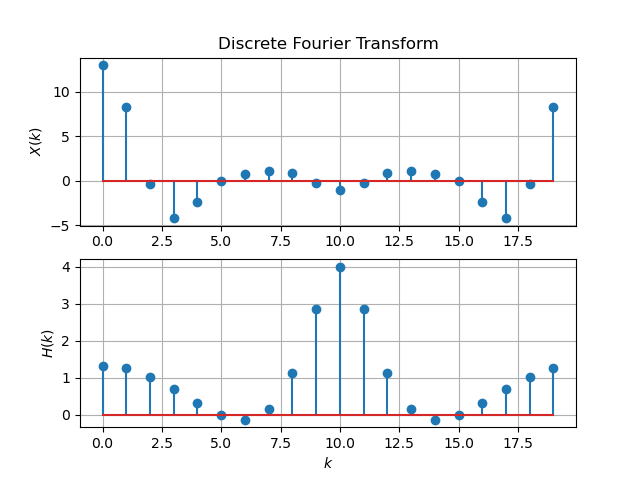
\includegraphics[width=\columnwidth]{./figs/6.1.png}
\caption{Plots of the real parts of the DFT of $x(n)$ and $h(n)$}
\label{fig:6.1}
\end{figure}

\item Compute 
\begin{equation}\label{6.2}
Y(k) = X(k)H(k)
\end{equation}
\solution Download and run the following code.
%
\begin{lstlisting}
wget https://github.com/jarpula-Bhanu/EE3900/blob/main/Filter/Codes/6.2.py
\end{lstlisting}
run the above code using the command.
\begin{lstlisting}
	python3 6.2.py
\end{lstlisting}

\item Compute
\begin{equation} \label{6.3}
 y\brak{n}={\frac {1}{N}}\sum _{k=0}^{N-1}Y\brak{k}\cdot e^{j 2\pi kn/N},\quad n = 0,1,\dots, N-1
\end{equation}
\\
\solution The following code plots Fig. \ref{fig:ynconv}. Note that this is the same as 
$y(n)$ in  Fig. 
\ref{fig:3.2}. 
%
\begin{lstlisting}
wget https://github.com/jarpula-Bhanu/EE3900/blob/main/Filter/Codes/6.3.py
\end{lstlisting}
run the above code using the command.
\begin{lstlisting}
	python3 6.3.py
\end{lstlisting}

\begin{figure}[!ht]
\centering
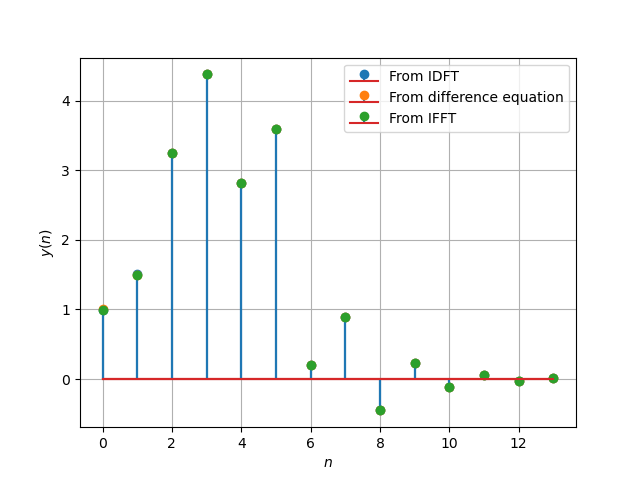
\includegraphics[width=\columnwidth]{./figs/6.3.png}
\caption{$y(n)$ from the DFT}
\label{fig:yndft}
\end{figure}

\item Repeat the previous exercise by computing $X(k), H(k)$ and $y(n)$ through FFT and 
 IFFT.
 \solution Download the code from
\begin{lstlisting}
wget https://github.com/jarpula-Bhanu/EE3900/blob/main/Filter/Codes/6.4.py
\end{lstlisting}
and execute it using
\begin{lstlisting}
$ python3 6.4.py
\end{lstlisting}
Observe that Fig. \eqref{fig:y-n-fft} is the same as $y(n)$ in Fig. \eqref{fig:3.2}.
\begin{figure}
\centering
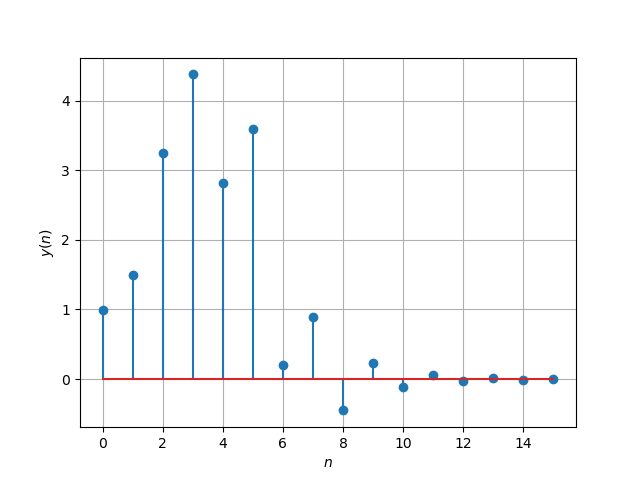
\includegraphics[width=\columnwidth]{figs/6.4.png}
\caption{$y(n)$ using FFT and IFFT}
\label{fig:y-n-fft}
\end{figure}
\item Wherever possible, express all the above equations as matrix equations.\\
\solution
We use the DFT Matrix, where $\omega = e^{-\frac{j2k\pi}{N}}$, which is given by
\begin{align}
	\mtx{W} = 
	\begin{pmatrix}
		\omega^0 & \omega^0 & \ldots & \omega^0 \\
		\omega^0 & \omega^1 & \ldots & \omega^{N - 1} \\
		\vdots & \vdots & \ddots & \vdots \\
		\omega^0 & \omega^{N - 1} & \ldots & \omega^{(N -1)(N - 1)}
	\end{pmatrix}
\end{align}
i.e. $W_{jk} = \omega^{jk}$, $0 \leq j, k < N$. Hence, we can write any DFT equation as
\begin{align}
	\mtx{X} = \mtx{W}\mtx{x} = \mtx{x}\mtx{W}
\end{align}
\noindent where
\begin{align}
	\mtx{x} = 
	\begin{pmatrix}
		x(0) \\ x(1) \\ \vdots \\ x(n - 1)
	\end{pmatrix}
\end{align}
\noindent Using \eqref{6.3}, the inverse Fourier Transform is given by
\begin{align}
	\mtx{x} = \mathcal{F}^{-1}\brak{\mtx{X}} = \mtx{W}^{-1}\mtx{X} &= \frac{1}{N}\mtx{W^{H}}\mtx{X} = \frac{1}{N}\mtx{X}\mtx{W^{H}} \\ 
	\implies \mtx{W}^{-1} &= \frac{1}{N}\mtx{W^{H}}
\end{align}
\noindent where $H$ denotes hermitian operator. We can rewrite \eqref{6.2} using the element-wise multiplication operator as
\begin{align}
	\mtx{Y} = \mtx{H}\cdot\mtx{X} = \brak{\mtx{W}\mtx{h}}\cdot\brak{\mtx{W}\mtx{x}}
\end{align}
\item Verify the above equation by generating the DFT matrix in python.\\
\solution Download the code from
\begin{lstlisting}
wget https://github.com/jarpula-Bhanu/EE3900/blob/main/Filter/Codes/6.6.py
\end{lstlisting}
and execute it using
\begin{lstlisting}
$ python3 6.6.py
\end{lstlisting}

The above code plots \eqref{fig:DFT matrix}
\begin{figure}
\centering
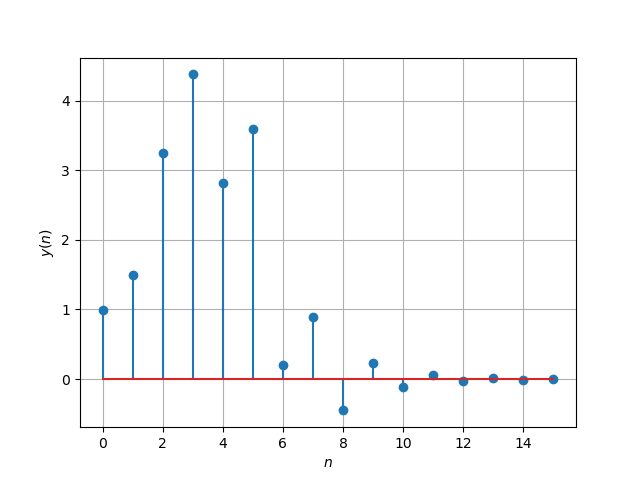
\includegraphics[width=\columnwidth]{figs/6.6.png}
\caption{$y(n)$ using DFT matrix}
\label{fig:DFT matrix}
\end{figure}

\item Compute the 8-point FFT in C.\\
\solution Download the following C code 
\begin{lstlisting}
wget https://github.com/jarpula-Bhanu/EE3900/blob/main/Filter/Codes/6.7.c
\end{lstlisting}
run the above C code using the command
\begin{lstlisting}
	$ gcc 6.7.c -lm -o 6.7.out
	$ ./6.7.out
\end{lstlisting}
The above code generates the text files that are loaded in the following code \\
Download the following code 
\begin{lstlisting}
wget https://github.com/jarpula-Bhanu/EE3900/blob/main/Filter/Codes/6.7.1_plot.py
wget https://github.com/jarpula-Bhanu/EE3900/blob/main/Filter/Codes/6.7.2_plot.py
\end{lstlisting}
run the above code using the command
\begin{lstlisting}
	$ python3 6.7.1_plot.py
	$ python3 6.7.2_plot.py
\end{lstlisting}
The above code plots the graphs \ref{fig:complexity fft/ifft} and \ref{fig:Complexity convolution}
\begin{figure}
\centering
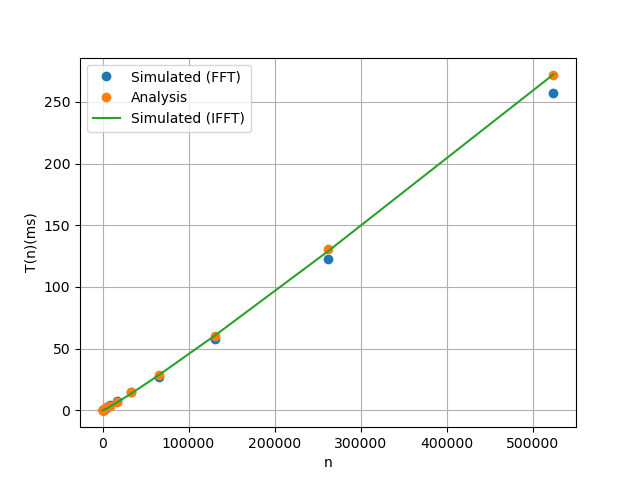
\includegraphics[width=\columnwidth]{figs/6.7.1_plot.png}
\caption{Complexity of FFT/IFFT is O(n log n)}
\label{fig:complexity fft/ifft}
\end{figure}

\begin{figure}
\centering
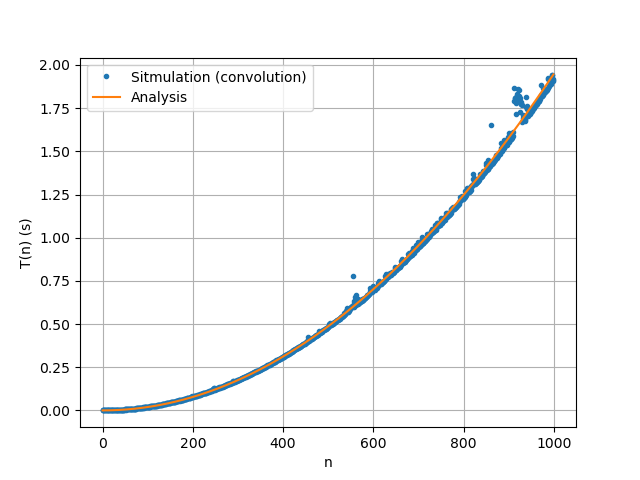
\includegraphics[width=\columnwidth]{figs/6.7.2_plot.png}
\caption{Complexity of convolution is O($n^2$)}
\label{fig:Complexity convolution}
\end{figure}
\end{enumerate}

\section{FFT}

\begin{enumerate}
    \item The DFT of $x(n)$ is given by
    \begin{align}
        X(k) \triangleq \sum_{n=0}^{N-1} x(n) e^{-j 2 \pi k n / N}, \quad k=0,1, \ldots, N-1
    \end{align}
\item Let 
	\begin{align}
W_{N} = e^{-j2\pi/N} 
	\end{align}
		Then the $N$-point {\em DFT matrix} is defined as 
	\begin{align}
		\vec{F}_{N} = \sbrak{W_{N}^{mn}}
	\end{align}
	where $W_{N}^{mn}$ are the elements of $\vec{F}_{N}$.
\item Let 
	\begin{align}
		\vec{I}_4 = \myvec{\vec{e}_4^{1} &\vec{e}_4^{2} &\vec{e}_4^{3} &\vec{e}_4^{4} }
	\end{align}
		be the $4\times 4$ identity matrix.  Then the 4 point {\em DFT permutation matrix} is defined as 
	\begin{align}
		\vec{P}_4 = \myvec{\vec{e}_4^{1} &\vec{e}_4^{3} &\vec{e}_4^{2} &\vec{e}_4^{4} }
	\end{align}
\item The 4 point {\em DFT diagonal matrix} is defined as 
	\begin{align}
		\vec{D}_4 = diag\myvec{W_{N}^{0} & W_{N}^{1} & W_{N}^{2} & W_{N}^{3}}
	\end{align}

\item Show that 
\begin{equation} \label{wwla}
    W_{N}^{2}=W_{N/2}
\end{equation}
\solution From defination
\begin{align}
	W_{N} &= e^{-j2\pi/N} \\
	W_{N}^2 &= \brak{e^{-j2\pi/N}}^2\\
	&= e^{-j2\pi/N/2}\\
	&=W_{N/2}
\end{align}

\item Show that 
\begin{equation}
	\vec{F}_{4}=
\begin{bmatrix}
	\vec{I}_{2} & \vec{D}_{2} \\
\vec{I}_{2} & -\vec{D}_{2}
\end{bmatrix}
\begin{bmatrix}
\vec{F}_{2} & 0 \\
0 & \vec{F}_{2}
\end{bmatrix}
\vec{P}_{4} 
\end{equation}
\solution \begin{align}
	\vec{F}_{4}\vec{P}_{4}&=
\begin{bmatrix}
	\vec{I}_{2} & \vec{D}_{2} \\
\vec{I}_{2} & -\vec{D}_{2}
\end{bmatrix}
\begin{bmatrix}
\vec{F}_{2} & 0 \\
0 & \vec{F}_{2}
\end{bmatrix}
\\
&=\begin{bmatrix}
	\vec{I}_{2}\vec{F}_{2} & \vec{D}_{2}\vec{F}_{2} \\
\vec{I}_{2}\vec{F}_{2} & -\vec{D}_{2}\vec{F}_{2}
\end{bmatrix}
\\
&= \begin{bmatrix}
	\vec{F}_{2} & \vec{D}_{2}\vec{F}_{2} \\
\vec{F}_{2} & -\vec{D}_{2}\vec{F}_{2}
\end{bmatrix}
\\
&=\begin{bmatrix}
	W_{2}^{0} &W_{2}^{0} &W_{2}^{0} &W_{2}^{0}\\
	W_{2}^{0} &W_{2}^{1} &W_{2}^{1} &W_{2}^{2}\\
	W_{2}^{0} &W_{2}^{0} &-W_{2}^{0} &-W_{2}^{0}\\
	W_{2}^{0} &W_{2}^{1} &-W_{2}^{1} &-W_{2}^{2}\\
\end{bmatrix}\\
&=\begin{bmatrix}
	1 &1 &1 &1\\
	1 &W_{2}^{1} &W_{2}^{1} &W_{2}^{2}\\
	1 &W_{2}^{0} &-W_{2}^{0} &-W_{2}^{0}\\
	1 &W_{2}^{1} &-W_{2}^{1} &-W_{2}^{2}\\
\end{bmatrix}
\end{align}
from eqn\eqref{wwla} we get $W_{2} = W_{4}^2$
\begin{align}
	\vec{F}_{4}\vec{P}_{4}&=\begin{bmatrix}
		W_{4}^{0}&W_{4}^{0}&W_{4}^{0}&W_{4}^{0}\\
		W_{4}^{0}&W_{4}^{2}&W_{4}^{1}&W_{4}^{3}\\
		W_{4}^{0}&W_{4}^{4}&W_{4}^{2}&W_{4}^{6}\\
		W_{4}^{0}&W_{4}^{6}&W_{4}^{3}&W_{4}^{9}\\
	\end{bmatrix}
\end{align}

\item Show that 
\begin{equation}
\vec{F}_{N}=
\begin{bmatrix}
\vec{I}_{N/2} & \vec{D}_{N/2} \\
\vec{I}_{N/2} & -\vec{D}_{N/2}
\end{bmatrix}
\begin{bmatrix}
\vec{F}_{N/2} & 0 \\
0 & \vec{F}_{N/2}
\end{bmatrix}
\vec{P}_{N}
\end{equation}
\solution  Observe that for even $N$ and letting $\vec{f}_N^i$ denote the $i^{\text{th}}$ column of $\vec{F}_N$, 
\begin{align}
	\myvec{\vec{D}_{N/2}\vec{F}_{N/2} \\ -\vec{D}_{N/2}\vec{F}_{N/2}} = \myvec{\vec{f}_N^{2} & \vec{f}_N^{4} & \ldots & \vec{f}_N^{N}}
\end{align}
and
\begin{align}
	\myvec{\vec{I}_{N/2}\vec{F}_{N/2} \\ \vec{I}_{N/2}\vec{F}_{N/2}} = \myvec{\vec{f}_N^{1} & \vec{f}_N^{3} & \ldots & \vec{f}_N^{N - 1}}
\end{align}
Thus,
\begin{align}
	&\myvec{\vec{I}_2\vec{F}_2 & \vec{D}_2\vec{F}_2 \\ \vec{I}_2\vec{F}_2 & -\vec{D}_2\vec{F}_2} = \myvec{\vec{I}_{N/2} & \vec{D}_{N/2} \\ \vec{I}_{N/2} & -\vec{D}_{N/2}}\myvec{\vec{F}_{N/2} & 0 \\ 0 & \vec{F}_{N/2}} \nonumber \\
	&= \myvec{\vec{f}_N^{1} & \ldots & \vec{f}_N^{N - 1} & \vec{f}_N^{2} & \ldots & \vec{f}_N^{N}}
\end{align}
and so,
\begin{align}
	&\myvec{\vec{I}_{N/2} & \vec{D}_{N/2} \\ \vec{I}_{N/2} & -\vec{D}_{N/2}}\myvec{\vec{F}_{N/2} & 0 \\ 0 & \vec{F}_{N/2}}\vec{P}_{N} \nonumber \\
	&= \myvec{\vec{f}_N^{1} & \vec{f}_N^{2} & \ldots & \vec{f}_N^{N}} = \vec{F}_N
\end{align}
\item Find 
    \begin{align}
	     \vec{P}_4 \vec{x}
    \end{align}
\solution  We have,
\begin{align}
	\vec{P}_4\vec{x} = \myvec{\vec{e}_4^1 & \vec{e}_4^3 & \vec{e}_4^2 & \vec{e}_4^4}\myvec{x(0)\\x(1)\\x(2)\\x(3)} = \myvec{x(0)\\x(2)\\x(1)\\x(3)}
	\label{eq:x-permute}
\end{align}
\item Show that 
    \begin{align}
	    \vec{X} = \vec{F}_N \vec{x}
	    \label{eq:dft-mat-def}
    \end{align}
		where $\vec{x}, \vec{X}$ are the vector representations of $x(n), X(k)$ respectively.\\
		\solution  Writing the terms of $X$, 
		\begin{align}
			X(0) &= x(0) + x(1) + \ldots + x(N - 1) \\
			X(1) &= x(0) + x(1)e^{-\frac{\j2\pi}{N}} + \ldots + \nonumber \\
				 &+ x(N - 1)e^{-\frac{\j2(N - 1)\pi}{N}} \\
				 &\vdots \nonumber \\
			X(N - 1) &= x(0) + x(1)e^{-\frac{\j2(N - 1)\pi}{N}} + \ldots + \nonumber \\
					 &+ x(N - 1)e^{-\frac{\j2(N - 1)(N - 1)\pi}{N}}	
		\end{align}
		Clearly, the term in the $m^{\text{th}}$ row and $n^{\text{th}}$ column is given by ($0 \leq m \leq N - 1$ and $0 \leq n \leq N - 1$) 
		\begin{align}
			T_{mn} = x(n)e^{-\frac{\j2mn\pi}{N}} 
		\end{align}
		and so, we can represent each of these terms as a matrix product
		\begin{align}
			\vec{X} = \vec{F}_N\vec{x}
		\end{align}
		where $\vec{F}_N = \sbrak{e^{-\frac{-\j2mn\pi}{N}}}_{mn}$ for $0 \leq m \leq N - 1$ and $0 \leq n \leq N - 1$.
\item Derive the following Step-by-step visualisation  of
8-point FFTs into 4-point FFTs and so on
\begin{equation}
\begin{bmatrix}
X(0) \\ 
X(1) \\ 
X(2) \\ 
X(3)
\end{bmatrix}
=
\begin{bmatrix}
X_{1}(0) \\ 
X_{1}(1)\\ 
X_{1}(2)\\
X_{1}(3)\\
\end{bmatrix}
+
\begin{bmatrix}
W^{0}_{8} & 0 & 0 & 0\\
0 & W^{1}_{8} & 0 & 0\\
0 & 0 & W^{2}_{8} & 0\\
0 & 0 & 0 & W^{3}_{8}
\end{bmatrix}
\begin{bmatrix}
X_{2}(0) \\ 
X_{2}(1) \\ 
X_{2}(2) \\
X_{2}(3)
\end{bmatrix}
\end{equation}
\begin{equation}
\begin{bmatrix}
X(4) \\ 
X(5) \\ 
X(6) \\ 
X(7)
\end{bmatrix}
=
\begin{bmatrix}
X_{1}(0) \\ 
X_{1}(1)\\ 
X_{1}(2)\\
X_{1}(3)\\
\end{bmatrix}
-
\begin{bmatrix}
W^{0}_{8} & 0 & 0 & 0\\
0 & W^{1}_{8} & 0 & 0\\
0 & 0 & W^{2}_{8} & 0\\
0 & 0 & 0 & W^{3}_{8}
\end{bmatrix}
\begin{bmatrix}
X_{2}(0) \\ 
X_{2}(1) \\ 
X_{2}(2) \\
X_{2}(3)
\end{bmatrix}
\end{equation}
4-point FFTs into 2-point FFTs
\begin{equation}
\begin{bmatrix}
X_{1}(0) \\ 
X_{1}(1)\\ 
\end{bmatrix}
=
\begin{bmatrix}
X_{3}(0) \\ 
X_{3}(1)\\ 
\end{bmatrix}
+
\begin{bmatrix}
W^{0}_{4} & 0\\
0 & W^{1}_{4}
\end{bmatrix}
\begin{bmatrix}
X_{4}(0) \\ 
X_{4}(1) \\ 
\end{bmatrix}
\end{equation}
\begin{equation}
\begin{bmatrix}
X_{1}(2) \\ 
X_{1}(3)\\ 
\end{bmatrix}
=
\begin{bmatrix}
X_{3}(0) \\ 
X_{3}(1)\\ 
\end{bmatrix}
-
\begin{bmatrix}
W^{0}_{4} & 0\\
0 & W^{1}_{4}
\end{bmatrix}
\begin{bmatrix}
X_{4}(0) \\ 
X_{4}(1) \\ 
\end{bmatrix}
\end{equation}
\begin{equation}
\begin{bmatrix}
X_{2}(0) \\ 
X_{2}(1)\\ 
\end{bmatrix}
=
\begin{bmatrix}
X_{5}(0) \\ 
X_{5}(1)\\ 
\end{bmatrix}
+
\begin{bmatrix}
W^{0}_{4} & 0\\
0 & W^{1}_{4}
\end{bmatrix}
\begin{bmatrix}
X_{6}(0) \\ 
X_{6}(1) \\ 
\end{bmatrix}
\end{equation}
\begin{equation}
\begin{bmatrix}
X_{2}(2) \\ 
X_{2}(3)\\ 
\end{bmatrix}
=
\begin{bmatrix}
X_{5}(0) \\ 
X_{5}(1)\\ 
\end{bmatrix}
-
\begin{bmatrix}
W^{0}_{4} & 0\\
0 & W^{1}_{4}
\end{bmatrix}
\begin{bmatrix}
X_{6}(0) \\ 
X_{6}(1) \\ 
\end{bmatrix}
\end{equation}
\begin{equation}
P_{8}
\begin{bmatrix}
x(0) \\ 
x(1) \\ 
x(2) \\ 
x(3) \\ 
x(4) \\ 
x(5) \\
x(6) \\
x(7)
\end{bmatrix}
 = 
\begin{bmatrix}
x(0) \\ 
x(2) \\ 
x(4) \\ 
x(6) \\
x(1) \\ 
x(3) \\ 
x(5) \\
x(7)
\end{bmatrix}
\end{equation}
\begin{equation}
P_{4}
\begin{bmatrix}
x(0) \\ 
x(2) \\ 
x(4) \\ 
x(6) \\
\end{bmatrix}
 = 
\begin{bmatrix}
x(0) \\ 
x(4) \\ 
x(2) \\
x(6)
\end{bmatrix}
\end{equation}
\begin{equation}
P_{4}
\begin{bmatrix}
x(1) \\ 
x(3) \\ 
x(5) \\
x(7)
\end{bmatrix}
 = 
\begin{bmatrix}
x(1) \\ 
x(5) \\ 
x(3) \\ 
x(7) \\
\end{bmatrix}
\end{equation}
Therefore,
\begin{equation}
\begin{bmatrix}
X_{3}(0) \\ 
X_{3}(1)\\ 
\end{bmatrix}
= F_{2}
\begin{bmatrix}
x(0) \\ 
x(4) \\ 
\end{bmatrix}
\end{equation}
\begin{equation}
\begin{bmatrix}
X_{4}(0) \\ 
X_{4}(1)\\ 
\end{bmatrix}
= F_{2}
\begin{bmatrix}
x(2) \\ 
x(6) \\ 
\end{bmatrix}
\end{equation}
\begin{equation}
\begin{bmatrix}
X_{5}(0) \\ 
X_{5}(1)\\ 
\end{bmatrix}
= F_{2}
\begin{bmatrix}
x(1) \\ 
x(5) \\ 
\end{bmatrix}
\end{equation}
\begin{equation}
\begin{bmatrix}
X_{6}(0) \\ 
X_{6}(1)\\ 
\end{bmatrix}
= F_{2}
\begin{bmatrix}
x(3) \\ 
x(7) \\ 
\end{bmatrix}
\end{equation}

\item For 
    \begin{align}
	    \vec{x} = \myvec{1\\2\\3\\4\\2\\1}
        \label{eq:equation1}
    \end{align}
    compte the DFT  
		using 
	    \eqref{eq:dft-mat-def}\\
\solution Download the code from
\begin{lstlisting}
wget https://github.com/jarpula-Bhanu/EE3900/blob/main/Filter/Codes/7.9.py
\end{lstlisting}
and execute it using
\begin{lstlisting}
$ python3 7.9.py
\end{lstlisting}

\item Repeat the above exercise using the FFT
after zero padding $\vec{x}$.\\
\solution Download the code from
\begin{lstlisting}
wget https://github.com/jarpula-Bhanu/EE3900/blob/main/Filter/Codes/7.10.py
\end{lstlisting}
and execute it using
\begin{lstlisting}
$ python3 7.10.py
\end{lstlisting}

\item Write a C program to compute the 8-point FFT.\\
\solution Download the code from
\begin{lstlisting}
wget https://github.com/jarpula-Bhanu/EE3900/blob/main/Filter/Codes/7.11.c
\end{lstlisting}
compile it using
\begin{lstlisting}
$ gcc 7.11.c -lm -o 7.11.out
\end{lstlisting}
and execute it using
\begin{lstlisting}
$ ./7.11.out
\end{lstlisting}
\begin{figure}[h]
	\centering
	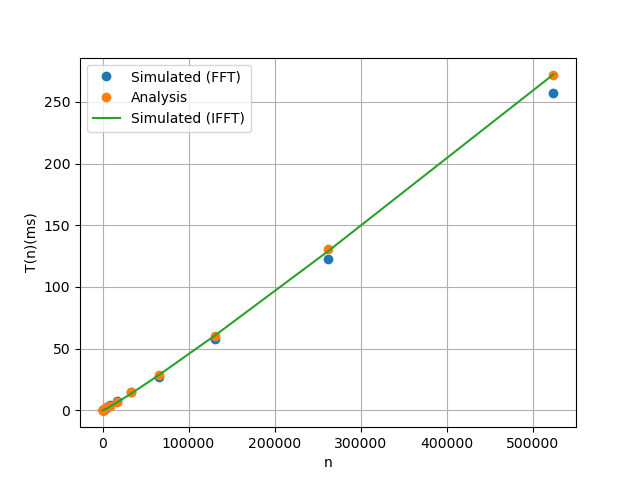
\includegraphics[width=\columnwidth]{figs/6.7.1_plot.png}
	\caption{Complexity of FFT/IFFT is O(n log n)}
	% \label{fig:complexity fft/ifft}
	\end{figure}
	
	\begin{figure}[h]
	\centering
	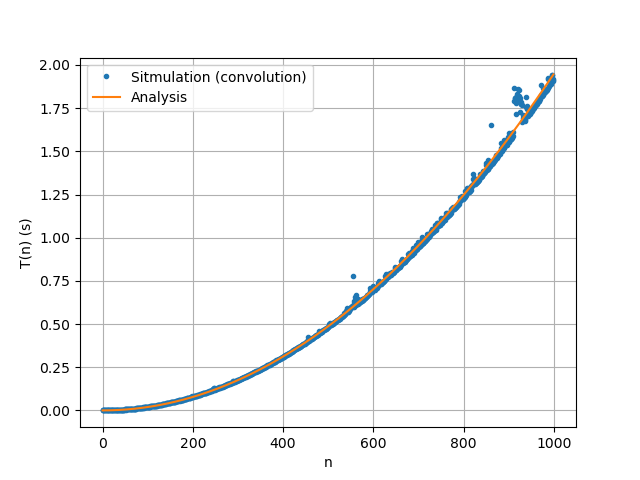
\includegraphics[width=\columnwidth]{figs/6.7.2_plot.png}
	\caption{Complexity of convolution is O($n^2$)}
	% \label{fig:Complexity convolution}
	\end{figure}

	\begin{figure}[h]
	\centering
	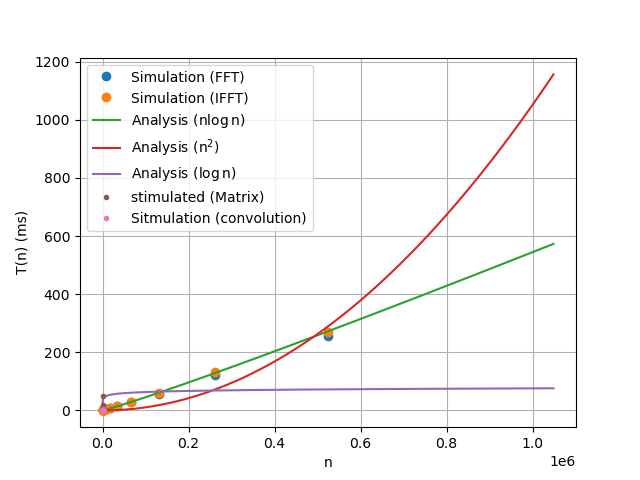
\includegraphics[width=\columnwidth]{figs/7_11.png}
	\caption{Comparision of complexities}
	% \label{fig:Complexity convolution}
	\end{figure}
	
 \end{enumerate}
\section{Exercises}
Answer the following questions by looking at the python code in Problem \ref{2.3}.
\begin{enumerate}[label=\thesection.\arabic*]
\item
The command
\begin{lstlisting}
	output_signal = signal.lfilter(b, a, input_signal)
	\end{lstlisting}
in Problem \ref{2.3} is executed through the following difference equation
\begin{equation}
\label{eq:iir_filter_gen}
 \sum _{m=0}^{M}a\brak{m}y\brak{n-m}=\sum _{k=0}^{N}b\brak{k}x\brak{n-k}
\end{equation}
%
where the input signal is $x(n)$ and the output signal is $y(n)$ with initial values all 0. Replace
\textbf{signal.filtfilt} with your own routine and verify.\\
\solution Download the code from
\begin{lstlisting}
wget https://github.com/jarpula-Bhanu/EE3900/blob/main/Filter/Codes/7.1.py
\end{lstlisting}
and execute it using
\begin{lstlisting}
$ python3 7.1.py
\end{lstlisting}
%
\item Repeat all the exercises in the previous sections for the above $a$ and $b$.\\
\solution For the given values, the difference equation is
\begin{align}
	&y(n) - \brak{4.44}y(n - 1) + \brak{8.78}y(n - 2) \nonumber \\
	&- \brak{9.93}y(n - 3) + \brak{6.90}y(n - 4) \nonumber \\
	&- \brak{2.93}y(n - 5) \nonumber + \brak{0.70}y(n - 6) \nonumber \\
	&- \brak{0.07}y(n - 7) = \brak{5.02 \times 10^{-5}}x(n) \nonumber \\
	&+ \brak{3.52 \times 10^{-4}}x(n - 1) + \brak{1.05 \times 10^{-3}}x(n - 2) \nonumber \\
	&+ \brak{1.76 \times 10^{-3}}x(n - 3) + \brak{1.76 \times 10^{-3}}x(n - 4) \nonumber \\
	&+ \brak{1.05 \times 10^{-3}}x(n - 5) + \brak{3.52 \times 10^{-4}}x(n - 6) \nonumber \\
	&+ \brak{5.02 \times 10^{-5}}x(n - 7)
\end{align}
From \eqref{eq:iir_filter_gen}, we see that the transfer function can be written as follows
\begin{align}
	H(z) &= \frac{\sum_{k = 0}^{N}b(k)z^{-k}}{\sum_{k = 0}^{M}a(k)z^{-k}} \\
		 &= \sum_{i}\frac{r(i)}{1 - p(i)z^{-1}} + \sum_{j}k(j)z^{-j}
	\label{eq:trans-func}
\end{align}
where $r(i)$, $p(i)$, are called residues and poles respectively of the partial 
fraction expansion of $H(z)$. $k(i)$ are the coefficients of the direct polynomial 
terms that might be left over. We can now take the inverse $z$-transform of
\eqref{eq:trans-func} and get using \eqref{eq:anun},
\begin{align}
	h(n) &= \sum_{i}r(i)[p(i)]^nu(n) + \sum_{j}k(j)\delta(n - j)
	\label{eq:h-n-expr}
\end{align}
Substituting the values,
\begin{align}
	&h(n) = [\brak{2.76}\brak{0.55}^n \nonumber \\ 
	&+ \brak{-1.05-1.84j}\brak{0.57+0.16j}^n \nonumber \\
	&+ \brak{-1.05+1.84j}\brak{0.57-0.16j}^n \nonumber \\
	&+ \brak{-0.53+0.08j}\brak{0.63+0.32j}^n \nonumber \\
	&+ \brak{-0.53-0.08j}\brak{0.63-0.32j}^n \nonumber \\
	&+ \brak{0.20+0.004j}\brak{0.75+0.47j}^n \nonumber \\
	&+ \brak{0.20-0.004j}\brak{0.75-0.47j}^n]u(n) \nonumber \\
	&+ \brak{-6.81 \times 10^{-4}}\delta(n)
\end{align}
The values $r(i)$, $p(i)$, $k(i)$ and thus the impulse response function are computed and plotted at
\begin{lstlisting}
wget https://github.com/jarpula-Bhanu/EE3900/blob/main/Filter/Codes/7.2.1.py
\end{lstlisting}
The filter frequency response is plotted at
\begin{lstlisting}
	wget https://github.com/jarpula-Bhanu/EE3900/blob/main/Filter/Codes/7.2.2.py
\end{lstlisting}
Observe that for a series $t_n = r^n$, $\frac{t_{n + 1}}{t_n} = r$.
By the ratio test, $t_n$ converges if $|r| < 1$. We observe that for all $i$, 
$|p(i)| < 1$ and so, as $h(n)$ is the sum of many convergent series,
we see that $h(n)$ converges and is bounded. From \eqref{eq:z_trans},
\begin{align}
	\sum_{n = 0}^{\infty}h(n) = H(1) = \frac{\sum_{k = 0}^{N}b(k)}{\sum_{k = 0}^{M}a(k)} = 1 < \infty
\end{align}
Therefore, the system is stable. From
Fig. \eqref{fig:butter-imp}, $h(n)$ is negligible after $n \geq 64$, and we
can apply a 64-bit FFT to get y(n). The following code uses the DFT matrix
to generate $y(n)$ in Fig. \eqref{fig:butter-out}.
\begin{lstlisting}
wget https://github.com/jarpula-Bhanu/EE3900/blob/main/Filter/Codes/7.2.3.py
\end{lstlisting}
The codes can be run all at once by typing
\begin{lstlisting}
$ python3 7.2.*.py
\end{lstlisting}
\begin{figure}[!htb]
	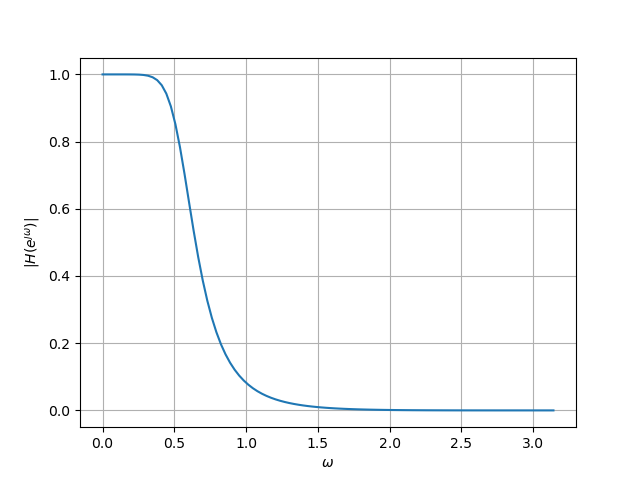
\includegraphics[width=\columnwidth]{figs/7.2.1.png}
	\caption{Plot of $h(n)$}
	\label{fig:butter-imp}
\end{figure}
\begin{figure}[!htb]
	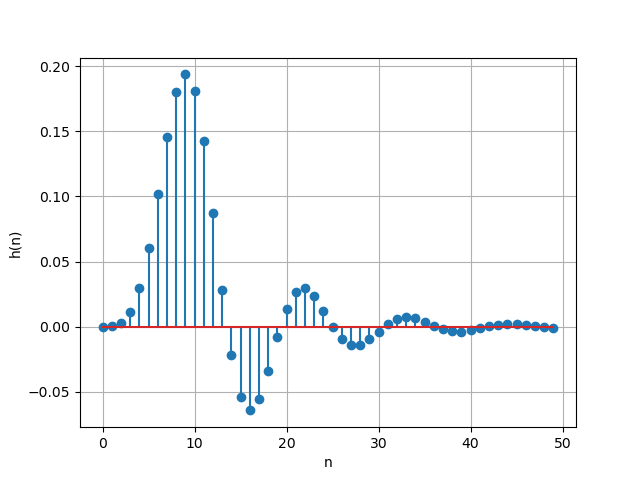
\includegraphics[width=\columnwidth]{figs/7.2.2.png}
	\caption{Filter frequency response}
	\label{fig:butter-resp}
\end{figure}
\begin{figure}[!htb]
	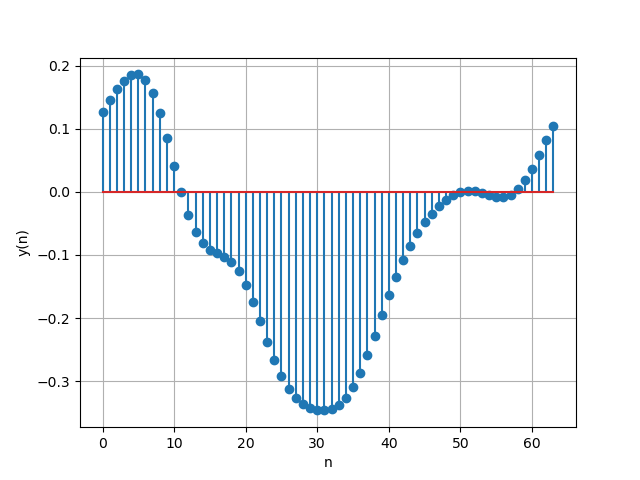
\includegraphics[width=\columnwidth]{figs/7.2.3.png}
	\caption{Plot of $y(n)$}
	\label{fig:butter-out}
\end{figure}

\item What is the sampling frequency of the input signal?
\\
\solution
Sampling frequency(fs)=44.1kHZ.
\item
What is type, order and  cutoff-frequency of the above butterworth filter
\\
\solution
The given butterworth filter is low pass with order=4 and cutoff-frequency=4kHz.
%
\item
Modifying the code with different input parameters and to get the best possible output.\\
%
\solution A better filtering was found on setting te order of the filter to be 7
\end{enumerate}

\end{document}